\documentclass[a4paper,onecolumn]{article}
\usepackage[width=180truemm,height=260truemm]{geometry}
\usepackage{amsmath}
\usepackage{amssymb}
\usepackage{amsfonts}
\usepackage{lmodern}
\usepackage{fourier}
\usepackage[T1]{fontenc}
\usepackage{graphicx}
\usepackage{algorithm}
\usepackage{algpseudocode}
\usepackage{fancyhdr}
\usepackage{lastpage}
\usepackage{indentfirst}

\pagestyle{fancy}
\lhead{}
\rhead{}
\cfoot{-- \thepage{}/{}\pageref{LastPage} --}
\renewcommand{\headrulewidth}{0pt}
\renewcommand{\footrulewidth}{0pt}

\newcommand{\bs}[1]{\boldsymbol{#1}}
\newcommand{\tran}{^{\mkern-1.5mu\mathsf{T}}}

\title{Gaussian Process Bootstrapping Layer}
\author{Tetsuya Ishikawa}

\begin{document}

\maketitle
\thispagestyle{fancy}

\section{Theoretical details}
% {{{

The Gaussian process with random Fourier features can be regarded as a variant of a fully connected layer.
We can design a new fully connected layer that can compute variance of it's intermediate features.

\subsection{Gaussian process with random Fourier features}

Let $\mathcal{D} = \{ (\boldsymbol{x}_n, y_n) \}_{n=1}^{N}$ be a training dataset where
$\boldsymbol{x}_n$ is a $n$-th data and $y_n$ is a label of $n$-th data.
The Gaussian process with random Fourier features can be formulated as follows:
\begin{align}
    \boldsymbol{\phi}_{\boldsymbol{x}_n}
    &= f(\boldsymbol{Wx}_n), \\
    \boldsymbol{P}
    &= \sum_{n = 1}^{N} \boldsymbol{\phi}_{\boldsymbol{x}_n}
    \boldsymbol{\phi}_{\boldsymbol{x}_n}^{\mkern-1.5mu\mathsf{T}}, \\
    m(\boldsymbol{x}_i)
    &= \frac{1}{\sigma^2} \boldsymbol{y}^{\mkern-1.5mu\mathsf{T}} \boldsymbol{\Phi}^{\mkern-1.5mu\mathsf{T}}
    \left( \boldsymbol{I} - (\boldsymbol{P} + \sigma^2 \boldsymbol{I})^{-1} \right) \boldsymbol{\phi}_{\boldsymbol{x}_i}, \\
    v(\boldsymbol{x}_i, \boldsymbol{x}_j)
    &= \boldsymbol{\phi}_{\boldsymbol{x}_i}^{\mkern-1.5mu\mathsf{T}} \left\{
    \boldsymbol{I} - \frac{1}{\sigma^2} \boldsymbol{P} \left( \boldsymbol{I} - (\boldsymbol{P} + \sigma^2 \boldsymbol{I})^{-1} \right)
    \right\} \boldsymbol{\phi}_{\boldsymbol{x}_j},
    \label{eqn:gp_variance}
\end{align}
where $f$ is a non-linear function and $\boldsymbol{W}$ is a random matrix derived from a kernel function of the Gaussian process.

\subsection{Analogy to a fully connected layer}

The formula $f(\boldsymbol{Wx})$ looks like a fully connected layer of neural network with activation function.
For example, if the kernel function is RBF kernel $k(\bs{x}_1, \bs{x}_2) = \exp \bigl( \| \bs{x}_1 - \bs{x}_2 \|^2 \bigr)$,
then $\boldsymbol{\phi}_{\boldsymbol{x}_n}$ can be written as
\begin{equation}
    \boldsymbol{\phi}_{\boldsymbol{x}_n} =
    \begin{pmatrix}
        \cos \bs{Wx}_n \\
        \sin \bs{Wx}_n
    \end{pmatrix},
    \hspace{10pt}
    \bs{W} \sim \mathcal{N} (0, \sigma^2).
\end{equation}
In this case, $\bs{Wx}_n$ corresponds to a fully connected layer and the 
circuler functions correspond to an activation function.

On the other hand, $v(\boldsymbol{x}_n, \boldsymbol{x}_n)$ correspond to the variance of input data $\boldsymbol{x}_n$.
Notable point is that the $v(\boldsymbol{x}_n, \boldsymbol{x}_n)$ is not depend on the label $y_n$,
in other words, variance $v(\boldsymbol{x}_n, \boldsymbol{x}_n)$ is the same for any label.
See the equation (\ref{eqn:gp_variance}).

\subsection{Gaussian process bootstrapping layer}

Bacause of the independence of the variance and $v(\boldsymbol{x}_n, \boldsymbol{x}_n)$ and the label $y_n$
mentioned in the previous subsection, we can replace the expectation prediction part as a identity function
(theoretically, this situation correspond that $y_n = \bs{\phi}_{\bs{x}_n}$). See the figure \ref{fig:sketch_gpbl}.
Therefore, we've got a new layer that can predict variance of intermediate features by replacing
the random Fourier features as a fully connected layer, and expectation prediction as a identity function.

Gaussian process bootstrapping layer is a layer to add noises to the intermediate features
where the variance of the noises is the variance of the intermediate features.  

\begin{figure}[t]
    \center
    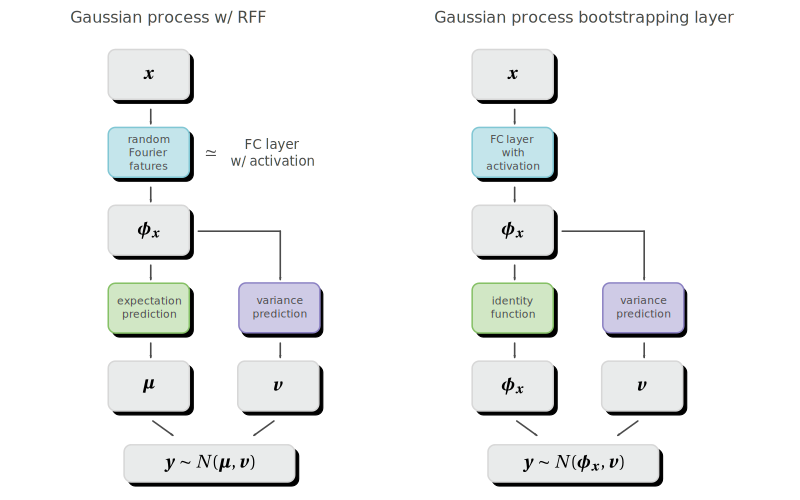
\includegraphics[width=300pt]{../figures/sketch_gpbl.pdf}
    \caption{Illustration of the analogy between GP w/ RFF and GPB layer}
    \label{fig:sketch_gpbl}
\end{figure}

\subsection{Psuedo code of GPB layer}

The algorithm \ref{alg:gpbl} is the pseudo code of the GPB layer.

\begin{algorithm}[t]
    \caption{Gaussian process bootstrapping layer}
    \label{alg:gpbl}
    \textbf{Input} \\
    \hspace*{\algorithmicindent}
    \begin{tabular}{rl}
        $\bs{X}$: & \hspace*{-10pt} tensor with shape $(N, C)$ \\
    \end{tabular} \\
    \textbf{Output} \\
    \hspace*{\algorithmicindent}
    \begin{tabular}{rl}
        $\bs{Y}$: & \hspace*{-10pt} tensor with shape $(N, C)$
    \end{tabular} \\
    \textbf{Hyperpatameters} \\
    \hspace*{\algorithmicindent}
    \begin{tabular}{rl}
        $\sigma$: & \hspace*{-10pt} standard deviation of measurement error \\
        $\alpha$: & \hspace*{-10pt} coefficient of exponential moving average \\
        $s$:      & \hspace*{-10pt} number of steps to skip bootstrapping \\
    \end{tabular} \\[10pt]
    \textbf{function}
    \textsc{Gaussian process bootstrapping layer}$(X, \alpha, \sigma)$ \\[5pt]
        \noindent\hspace*{\algorithmicindent}
        \texttt{\# Update matrix P with exponential moving average.} \\[1pt]
        \noindent\hspace*{\algorithmicindent}
        $\bs{P} = \alpha \bs{X}\tran \bs{X} + (1 - \alpha) \bs{P}$ \\

        \vspace*{-6pt}
        \noindent\hspace*{\algorithmicindent}
        \texttt{\# Compute matrix M.} \\[1pt]
        \noindent\hspace*{\algorithmicindent}
        $\bs{M} = \bs{I} - \frac{1}{\sigma^2} \bs{P} \bigl( \bs{I} - (\bs{P} + \sigma^2 * \bs{I})^{-1} \bs{P} \bigr)$ \\

        \vspace*{-6pt}
        \noindent\hspace*{\algorithmicindent}
        \texttt{\# Compute variance v[n].} \\[1pt]
        \noindent\hspace*{\algorithmicindent}
        $\textbf{for} \,\, n \,\, \textbf{in} \,\, [0, N):$ \\
        \noindent\hspace*{\algorithmicindent}\hspace*{\algorithmicindent}
        $v[n] = X[n, :]\tran M X[n, :]$ \\

        \vspace*{-6pt}
        \noindent\hspace*{\algorithmicindent}
        \texttt{\# Add perturbation to the input tensor X.} \\[1pt]
        \noindent\hspace*{\algorithmicindent}
        $\textbf{for} \,\, n \,\, \textbf{in} \,\, [0, N):$ \\
        \noindent\hspace*{\algorithmicindent}\hspace*{\algorithmicindent}
        $Y[n, :] = X[n, :] + \sqrt{v[n]} \, \bigl( \textrm{sampling from normal distribution with shape} \,\, (1, C) \bigr)$ \\[5pt]
    \textbf{end function}
 
\end{algorithm}

% }}}

\begin{thebibliography}{9}
% {{{

    \bibitem{Rasmussen2006}
        C. Rasmussen and C. Williams, “Gaussian Processes for Machine Learning”, MIT Press, 2006.

    \bibitem{Rahimi2007}
        A. Rahimi and B. Recht, "Random Features for Large-Scale Kernel Machines", NIPS, 2007.

% }}}
\end{thebibliography}

\end{document}


% vim: expandtab tabstop=4 shiftwidth=4 fdm=marker
